\documentclass[
  bibliography=totoc,     % Literatur im Inhaltsverzeichnis
  captions=tableheading,  % Tabellenüberschriften
  titlepage=firstiscover, % Titelseite ist Deckblatt
]{scrartcl}

% Paket float verbessern
\usepackage{scrhack}

% Warnung, falls nochmal kompiliert werden muss
\usepackage[aux]{rerunfilecheck}

% unverzichtbare Mathe-Befehle
\usepackage{amsmath}
% viele Mathe-Symbole
\usepackage{amssymb}
% Erweiterungen für amsmath
\usepackage{mathtools}

% Fonteinstellungen
\usepackage{fontspec}
% Latin Modern Fonts werden automatisch geladen
% Alternativ zum Beispiel:
%\setromanfont{Libertinus Serif}
%\setsansfont{Libertinus Sans}
%\setmonofont{Libertinus Mono}

% Wenn man andere Schriftarten gesetzt hat,
% sollte man das Seiten-Layout neu berechnen lassen
\recalctypearea{}

% deutsche Spracheinstellungen
\usepackage[ngerman]{babel}


\usepackage[
  math-style=ISO,    % ┐
  bold-style=ISO,    % │
  sans-style=italic, % │ ISO-Standard folgen
  nabla=upright,     % │
  partial=upright,   % │
  mathrm=sym,        % ┘
  warnings-off={           % ┐
    mathtools-colon,       % │ unnötige Warnungen ausschalten
    mathtools-overbracket, % │
  },                       % ┘
]{unicode-math}

% traditionelle Fonts für Mathematik
\setmathfont{Latin Modern Math}
% Alternativ zum Beispiel:
%\setmathfont{Libertinus Math}

\setmathfont{XITS Math}[range={scr, bfscr}]
\setmathfont{XITS Math}[range={cal, bfcal}, StylisticSet=1]

% Zahlen und Einheiten
\usepackage[
  locale=DE,                   % deutsche Einstellungen
  separate-uncertainty=true,   % immer Unsicherheit mit \pm
  per-mode=symbol-or-fraction, % / in inline math, fraction in display math
]{siunitx}

% chemische Formeln
\usepackage[
  version=4,
  math-greek=default, % ┐ mit unicode-math zusammenarbeiten
  text-greek=default, % ┘
]{mhchem}

% richtige Anführungszeichen
\usepackage[autostyle]{csquotes}

% schöne Brüche im Text
\usepackage{xfrac}

% Standardplatzierung für Floats einstellen
\usepackage{float}
\floatplacement{figure}{htbp}
\floatplacement{table}{htbp}

% Floats innerhalb einer Section halten
\usepackage[
  section, % Floats innerhalb der Section halten
  below,   % unterhalb der Section aber auf der selben Seite ist ok
]{placeins}

% Seite drehen für breite Tabellen: landscape Umgebung
\usepackage{pdflscape}

% Captions schöner machen.
\usepackage[
  labelfont=bf,        % Tabelle x: Abbildung y: ist jetzt fett
  font=small,          % Schrift etwas kleiner als Dokument
  width=0.9\textwidth, % maximale Breite einer Caption schmaler
]{caption}
% subfigure, subtable, subref
\usepackage{subcaption}

% Grafiken können eingebunden werden
\usepackage{graphicx}

% schöne Tabellen
\usepackage{tabularray}
\UseTblrLibrary{booktabs, siunitx}

% Verbesserungen am Schriftbild
\usepackage{microtype}

% Literaturverzeichnis
\usepackage[
  backend=biber,
]{biblatex}
% Quellendatenbank
\addbibresource{lit.bib}
\addbibresource{programme.bib}

% Hyperlinks im Dokument
\usepackage[
  german,
  unicode,        % Unicode in PDF-Attributen erlauben
  pdfusetitle,    % Titel, Autoren und Datum als PDF-Attribute
  pdfcreator={},  % ┐ PDF-Attribute säubern
  pdfproducer={}, % ┘
]{hyperref}
% erweiterte Bookmarks im PDF
\usepackage{bookmark}

% Trennung von Wörtern mit Strichen
\usepackage[shortcuts]{extdash}

\author{%
  Vincent Wirsdörfer\\%
  \href{mailto:vincent.wirsdoerfer@udo.edu}{authorA@udo.edu}%
  \and%
  Joris Daus\\%
  \href{mailto:joris.daus@udo.edu}{authorB@udo.edu}%
}
\publishers{TU Dortmund – Fakultät Physik}


\begin{document}

\section{Zielsetzung}
\label{sec:Zielsetzung}

Das Ziel des im folgend protokollierten Versuchs besteht darin die Elementarladung $e_0$ eines Elektrons
zu bestimmen. Dazu wird die Öltröpfchenmethode von Robert Andrew Millikan durchgeführt.

\section{Theorie}
\label{sec:Theorie}

Zum Zwecke der Bestimmung der Elementarladung werden feine Öltröpfchen in das vertikale und approximativ 
homogene elektrische Feld eines Plattenkondensators zerstäubt. Bei diesem Vorgang werden die Tröpfchen
aufgrund von Reibung elektrisch geladen. Zudem wirken bei abgeschaltetem Kondensator zwei Kräfte auf die 
Öltröpfchen. Zum einen bewegt sich ein Tröpfchen der Masse $m$ angesichts der Gravitationskraft
$\vec{F}_\text{G} = m\vec{g}$ nach unten, zum anderen bewirkt die Viskosität der Luft $\eta_\text{L}$ eine 
Reibungskraft $\vec{F}_\text{R} = -6\pi{}r\eta{}_\text{L}\vec{v}$ entgegen der Bewegungsrichtung der Masse. 
Hierbei bezeichnet $r$ den Radius eines Öltröpfchens. Wenn das Tröpfchen nach einer Phase der Beschleunigung 
eine konstante Geschwindigkeit $v_0$ annimmt, gilt das Kräftegleichgewicht

\begin{equation}
\label{eqn:Gewicht1}
    \frac{4\pi}{3}r³\left(\rho_\text{Oel}-\rho_\text{L}\right)g = 6\pi{}\eta_\text{L}rv_0.
\end{equation}

\noindent Der Korrekturterm $\rho_\text{L}$ repräsentiert den Auftrieb, den das Öltröpfchen bei der
Fallbewegung erhält. Nach Umstellen der Gleichung \eqref{eqn:Gewicht1} folgt der Tröpfchenradius:

\begin{equation*}
%\label{eqn:Radius}
    r = \sqrt{\frac{9\eta_\text{L}v_0}{2g\left(\rho_\text{Oel}-\rho_\text{L}\right)}}
\end{equation*}

\noindent Beim Anschluss des Kondensators an eine Spannungsquelle entsteht ein, je nach Polung, gerichtetes 
elektrisches Feld $\vec{E}$. Dieses Feld bewirkt eine zusätzliche elektrische Kraft $\vec{F}_\text{el} = g\vec{E}$
auf die Öltröpfchen, welche abhängig von der Polung der Platten über die Bewegungsrichtung der Tröpfchen entscheidet.
Diese Situation wird in Abbildung \ref{fig:GewichtV} veranschaulicht.

\begin{figure}
    \centering
    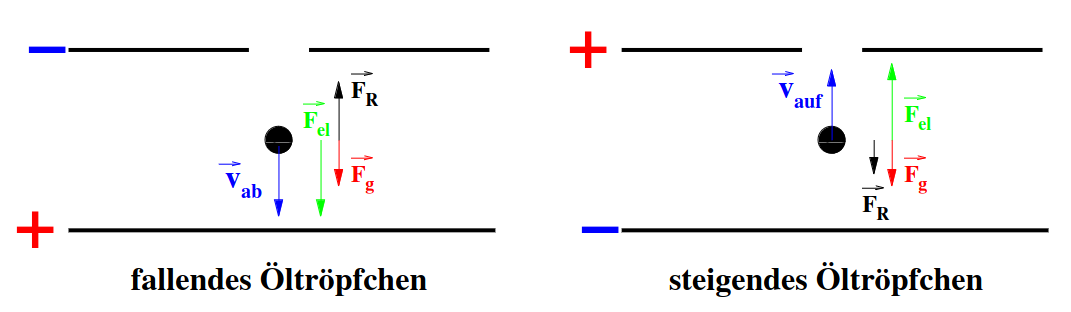
\includegraphics[width=\textwidth]{GewichtV.png}
    \caption{Gleichgewichtslage eines Öltröpfchens im homogenen E-Feld \cite{Versuchsanleitung_v503}.}
    \label{fig:GewichtV}
\end{figure}

\noindent Bei einer positiv geladenen unteren Platte wirkt die elektrische Kraft $\vec{F}_\text{el}$
in Richtung der Gravitationskraft. Dementsprechend sinken die Öltröpfchen mit einer Geschwindigkeit $\vec{v}_\text{ab}$
nach unten, was die Kräftegleichung 

\begin{equation}
\label{eqn:Gewicht2}
    \frac{4\pi}{3}r³\left(\rho_\text{Oel}-\rho_\text{L}\right)g - 6\pi{}\eta_\text{L}rv_\text{ab} = -qE
\end{equation}

\noindent zur Folge hat. Bei entgegengesetztem elektrischen Feld steigen die Tröpfchen auf, weshalb die
elektrische Kraft der Gravitation und Reibung entgegenwirkt. Die Kräftegleichung ändert sich somit zu 

\begin{equation}
\label{eqn:Gewicht3}
\frac{4\pi}{3}r³\left(\rho_\text{Oel}+\rho_\text{L}\right)g + 6\pi{}\eta_\text{L}rv_\text{ab} = qE.
\end{equation}

\noindent Aus den Gleichungen \eqref{eqn:Gewicht2} und \eqref{eqn:Gewicht3} folgt der Ausdruck

\begin{equation}
\label{eqn:Ladung}
    q = 3\pi{}\eta_\text{L}\sqrt{\frac{9\eta_\text{L}\left(v_\text{ab}-v_\text{auf}\right)}{4g\left(\rho_\text{Oel}-\rho_\text{L}\right)}}\cdot\frac{\left(v_\text{ab}+v_\text{auf}\right)}{E}
\end{equation}

\noindent für die Ladung und daraus

\begin{equation}
\label{eqn:Radius}
    r = \sqrt{\frac{9\eta_\text{L}\left(v_\text{ab}-v_\text{auf}\right)}{2g\left(\rho_\text{Oel}-\rho_\text{L}\right)}}
\end{equation}

\noindent für den Tröpfchenradius.\\

\noindent Zuletzt muss jedoch angebracht werden, dass die Stokes'sche Reibung ausschließlich für Tröpfchen gilt, deren Abmessung
größer als die mittlere freie Weglänge $\bar{l}$ in Luft ist. Diese Voraussetzung kann jedoch nicht ohne Weiteres
angenommen werden, weshalb die Viskosität $\eta_\text{L}$ von Luft durch den \emph{Cunningham-Korrekturterm} 

\begin{equation*}
%\label{eqn:cunningVisk}
    \eta_\text{eff} = \eta_\text{L}\left(\frac{1}{1 + \frac{B}{pr}}\right)
\end{equation*}

\noindent verändert werden muss. Hierbei ist $B = 822.599\cdot{}10{-5}\,\unit{\pascal\meter}$. Daraus folgt die korrigierte 
Ladung $q_\text{eff}$ mit 

\begin{equation}
\label{eqn:cunningLad}
    q_\text{eff} = q\left(\frac{1}{\left(1+\frac{B}{pr}\right)^{\frac{3}{2}}}\right).
\end{equation}

\end{document}